\section{Numerische Integration}
Ziel: Näherungsweise Berechnung von bestimmten Integralen
durch ``Quadraturformeln'', z.B. durch:
\begin{align*}
  \int_a^b f(x) \dx \simeq I_{[a,b]]}^{(n)}(f) := \sumizn{w_i f(x_i)}
\end{align*}
wobei $w_i$ Integrationsgewichte und $x_i$ Stützstellen sind.
\para{Definition:} Der Genauigkeitsgrad einer QF $I_{[a,b]}^{(n)}$ ist
die größte Zahl $r \in \mathbb{N}_0$, für die gilt:
\begin{align*}
  \int_a^b f(x) \dx = I_{[a,b]}^{(n)}(p)\,\forall\,p \in \Pi_r
\end{align*}

\subsection{Interpolatorische Quadraturformeln 1 (IQF)}
Konstruktion der QF über Interpolation von $f$ in $a \leq x_0 < \ldots < x_n \leq b$.
\begin{align*}
  \int_a^b f(x) \dx &\approx \int_a^b \underbrace{p_r(x)}_{\text{IP}} \dx = 
  \int_a^b \sumizn{f(x_i)L_i(x)\dx} = \sumizn{f(x_i) \int_a^b L_i(x)\dx} \tag{4.1}\\
  &= \sumizn{f(x_i) \int_a^b \prod_{j=0,i\neq j}^n \frac{x-x_j}{x_i - x_j}\dx}
\end{align*}
$w_i$ sind nicht abhängig von $f$. Fehler von (4.1.):
\begin{align*}
  \abs{\int_a^b f(x)\dx - \int_a^b p_n(x)\dx} &= \abs{ \int_a^b \frac{1}{(n+1)!} f^{(n+1)}(\xi(x))(x-x_0)\cdots(x-x_n)\dx}\\
  &\leq \frac{1}{(n+1)!} \norm{f^{(n+1)}}_\infty \underbrace{\norm{(x-x_0)\cdots(x-x_n)}_\infty}_{(b-a)^{n+1}} \underbrace{\int_a^b 1 \dx}_{b-a}\\
  &\leq \frac{\norm{f^{(n+1)}}_\infty}{(n+1)!}(b-a)^{n+2}
\end{align*}
Genauigkeitsgrad einer IQF $I_{[a,b]}^{(n)}$: mindestens $n$

\subsubsection{Geschlossene Newton-Cotes-Formeln}
Sind IQF mit gleichmäßig verteilten Stützstellen $x_i = a + ih$ $i=0,\ldots,n$ $h=\frac{b-a}{n}$.
(``Geschlossen'', weil $a$ und $b$ als Stützstellen verwendet werden.)\\
Beispiel: $n=1$ $x_0=a$ $x_1=b$
\begin{figure}[htbp]
  \centering
  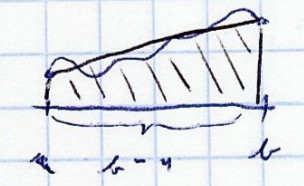
\includegraphics[width=0.3\textwidth]{figures/bsp_g_ncf.png}
  \caption{Geschlossene Newton-Cotes-Formel für $n=1$}
\end{figure}
\begin{align*}
  \int_a^b f(x) \dx \approx \frac{1}{2} (b-a)[f(a)+f(b)] \tag{Trapezregel}\\
  w_0 = w_1 = \frac{1}{2} (b-a)
\end{align*}
Integrationsgewichte ($n$ allgemein)
\begin{align*}
  w_i &= \int_a^b L_i(x) \dx = \int_a^b \prod_{j=0,i\neq j}^n \frac{x-x_j}{x_i - x_j}\dx =\\
  &= h \int_{t(a) = 0}^{t(b) = n} \frac{a + th - (a+jh)}{a + ih - (a+jh)} \dvar{t} = h \int_0^t \prod \frac{(t-j)h}{i-j)h} \dvar{t}
\end{align*}
\begin{align*}
  t:= \frac{x-a}{h} && \frac{\dvar{t}}{\dx} = \frac{1}{h} \\
  t(a)=0 && t(b)=\frac{b-a}{h}=n && x_j = n + jh
\end{align*}

\subsubsection{Offene Newton-Cotes-Formeln}
Sind IQF mit $x_i = a + (i+1)h$ $i=0,\ldots,n \in \mathbb{N}_0$
$h=\frac{b-a}{n+2}$
\begin{figure}[htbp]
  \centering
  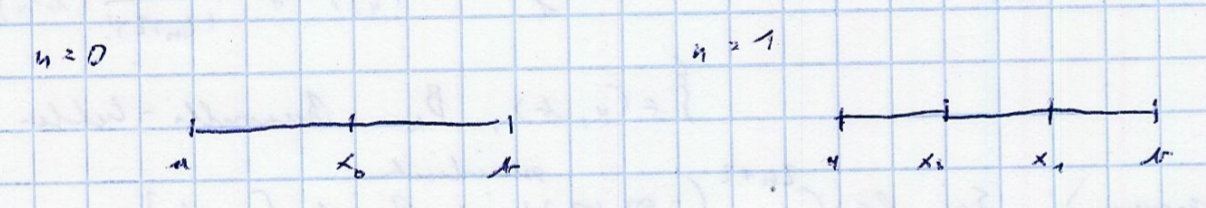
\includegraphics[width=0.7\textwidth]{figures/o_ncf.png}
  \caption{Stützstellen für offene Newton-Cotes-Formel für $n=0$ und $n=1$}
\end{figure}
\begin{figure}[htbp]
  \centering
  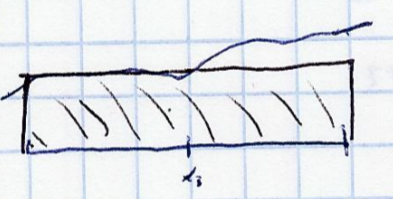
\includegraphics[width=0.3\textwidth]{figures/bsp_o_ncf.png}
  \caption{Offene Newton-Cotes-Formel für $n=0$}
\end{figure}
Beispiel: $n=0$
\begin{align*}
  \int_a^b f(x) \dx \approx \underbrace{(b-a)}_{w_0} f(\frac{a+b}{2}) \tag{Mittelpunkt-/Rechteckregel}
\end{align*}
Warnung: Bei Newton-Cotes-Formeln treten bei $n \geq 8$ (geschlossene) und $n \geq 2$ (offene)
negative Gewichte auf, was zur Auslöschung führen kann. (Oft: $f \geq 0$ oder $f \leq 0$).
Daher für solche $n$ nie verwenden.

\subsection{Summierte Quadraturformeln}
Idee: Unterteile $[a,b]$ in $N$ Teilintervalle. Wende auf jedem Teilintervall vorgebene QF an.
Sinnvoll (notwendig): Fehler hängt von $(b-a)$ ab.
\para{Summierte Trapezregel}
Unterteile $[a,b]$ in $N$ Teilintervalle der Länge $h=\frac{b-a}{N}$ $x_i := a + ih$ $i=0,\ldots,N$.
\begin{align*}
  \int_a^b f(x) \dx &= \sum^{N}_{i=1} \int_{x_{i-1}}^{x_i} f(x) \dx\\
  &\approx \sum^{N}_{i=1} \frac{h}{2} \left[f(x_{i-1}) + f(x_i)\right] \\
  &= h\left[\frac{1}{2} f(a) + \sum^{N-1}_{i=1} f(x_i) + \frac{1}{2} f(b)\right] =: I_h^{(1)}(f)
\end{align*}
\para{Summierte Simpsonregel}
\begin{figure}[htbp]
  \centering
  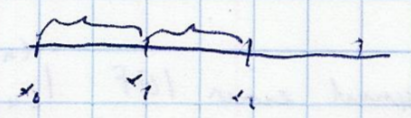
\includegraphics[width=0.5\textwidth]{figures/sum_simpson.png}
  \caption{Summierte Simpsonregel}
\end{figure}
\begin{align*}
  \int_a^b f(x) \dx &= \sum^{N}_{i=1} \int_{x_{i-1}}^{x_i} f(x) \dx\\
  &\approx \sum^{N}_{i=1} \frac{h}{6} \left[f(x_{i-1}) + 4f(\frac{x_{i-1}+x_i}{2}) + f(x_i)\right] \\
  &= \frac{h}{6} \left[ f(a) + 2 \sum^{N-1}_{i=1} f(x_i) + 4 \sum^{N}_{i=1} \frac{x_{i-1}+x_i}{2} + f(b) \right] := I_h^{(2)}(f)
\end{align*}
\para{Satz:}
\begin{enumerate}[a)]
  \item Für $f \in C^2[a, b]$ gilt: \begin{align*}
    \abs{\int_a^b f(x) \dx - I_h^{(1)}(f)} \leq ch^2 (b-a) \norm{f''}_\infty \underset{n \to \infty}{\longrightarrow} 0
  \end{align*}
  \item Für $f \in C^4[a, b]$ gilt: \begin{align*}
      \abs{\int_a^b f(x) \dx - I_h^{(2)}(f)} \leq ch^4 (b-a) \norm{f^{(4)}}_\infty \underset{n \to \infty}{\longrightarrow} 0
  \end{align*}
\end{enumerate}
Beweis für a):
\begin{align*}
  \abs{\int_a^b f(x) \dx - I_h^{(1)}(f)} \leq c \sum^{N}_{i=1} h^3 \norm{f''}_\infty = c \underbrace{h^3}_{\frac{(b-a)^3}{N^3}} N \norm{f''}_\infty = c h^2 (b-a) \norm{f''}_\infty
\end{align*}

\subsection{Euler-Maclaurinsche Summenformel}
Ziel: Genauigkeit der summierten Trapezregel ist erhöht bzw. kann erhöht werden.
\para{Satz:} Sei $f \in C^{2m+2}[a,b]$. Dann gilt
\begin{align*}
  I_h^{(1)}(f) = \int_a^b f(x) \dx + \sum^{m}_{k=1} h^{2k} \frac{B_k}{(2k)!} \left(f^{(2k-1)}(b) -
  f^{(2k-1)}(a)\right) + h^{2m+2}\frac{B_{2m+2}}{(2m+2)!} f^{(2m+2)}(\xi)
\end{align*}
$\xi \in (a,b)$, $B_k$ Bernoulli-Zahlen\\
Korollar (unmittelbare Konsequenz): Sei $f \in C^{2m+2}(-\infty, \infty)$ periodisch mit Periode $[a,b]$.
Dann ist $f^{(k)}(a) = f^{(k)}(b)$ für $k=0,\ldots,2m+2$ und 
$I_h^{(1)} - \int_a^b f(x) \dx = \LandauO(h^{2m+2})$.

\subsubsection{Romberg-Integrationsverfahren}
\begin{align*}
  I := \int_a^b f(x) \dx && T(h) := I_h^{(1)}\\
  I-T(h) &= c_1h^2 + c_2h^4+c_3h^6+\ldots+\LandauO(h^{2m+2})\\
  I-T(\frac{h}{2}) &= \frac{c_1}{4} h^2 + c_2^1h^4+\ldots+\LandauO(h^{2m+2})\\
  I-[\frac{4}{3} \underbrace{T(\frac{h}{2})}_{\LandauO(\frac{h^2}{4}} - \frac{1}{3} \underbrace{T(h)}_{\LandauO(h^2)} ] &= \tilde{c}_2h^4 + \tilde{c}_3h^6 + \ldots + \LandauO(h^{2m+2})
\end{align*}
Also: Kenne ich $T(h)$ und $T(\frac{h}{2})\rightarrow$ Fehler $\LandauO(h^4)$
\begin{align*}
  T_1(h) :&= \frac{4}{3} T(\frac{h}{2}) - \frac{1}{3} T(h) = \tilde{c}_2h^4 + \tilde{c}_3h^6 + \ldots + \LandauO(h^{2m+2})\\
  T_1(\frac{h}{2}) &= \frac{\tilde{c}_2}{16} h^4 + \hat{c}_3 h^6 + \ldots + \LandauO(h^{2m+2})\\
  T_1(\frac{h}{2}) &= \frac{4}{3} T(\frac{h}{4}) - \frac{1}{3} T(\frac{h}{2})\\
  I-\underbrace{[\frac{16}{15} T_1(\frac{h}{2}) - \frac{1}{15} T_1(h)]}_{=: T_2(h)} &= \breve{c}_3 h^6 + \ldots + \LandauO(h^{2m+2})
\end{align*}
Romberg-Schema $T_0(h) := T(h)$
\begin{align*}
  \begin{matrix}
    T_0(h)                & \searrow    & \LandauO(h^4)    &             &               &           &\\
    T_0(\frac{h}{2})      & \rightarrow & T_1(h)           & \searrow    & \LandauO(h^6) &           &\\
    T_0(\frac{h}{4})      & \esearrow & T_1(\frac{h}{2}) & \rightarrow & T_2(h)        &  \ddots     &\\
    \vdots                &             &                  &             &               &           & \LandauO(h^{2m+2})\\
    T_0(\frac{h}{2^m})    & \ldots      & \ldots           & \ldots      &      \ldots   &  \ldots   & T_m(h) \\ % TODO richtig laut mitschrift T_m(m^6)???
  \end{matrix}
\end{align*}
\begin{align*}
  T_k\left(\frac{h}{2^i}\right) = \left( 4^k T_{k-1}\left(\frac{h}{2^{i+1}} \right) - T_{k-1}\left(\frac{h}{2^i} \right) \right) \left(4^k-1\right)^{-1}
\end{align*}
\para{Satz:} Sei $f \in C^{2m+2}[a,b] \Rightarrow \abs{I-T_m(h)} = \LandauO\left(\left[\frac{h}{2^m} \right]^{2m+2} \right)$
\begin{figure}[htbp]
  \centering
  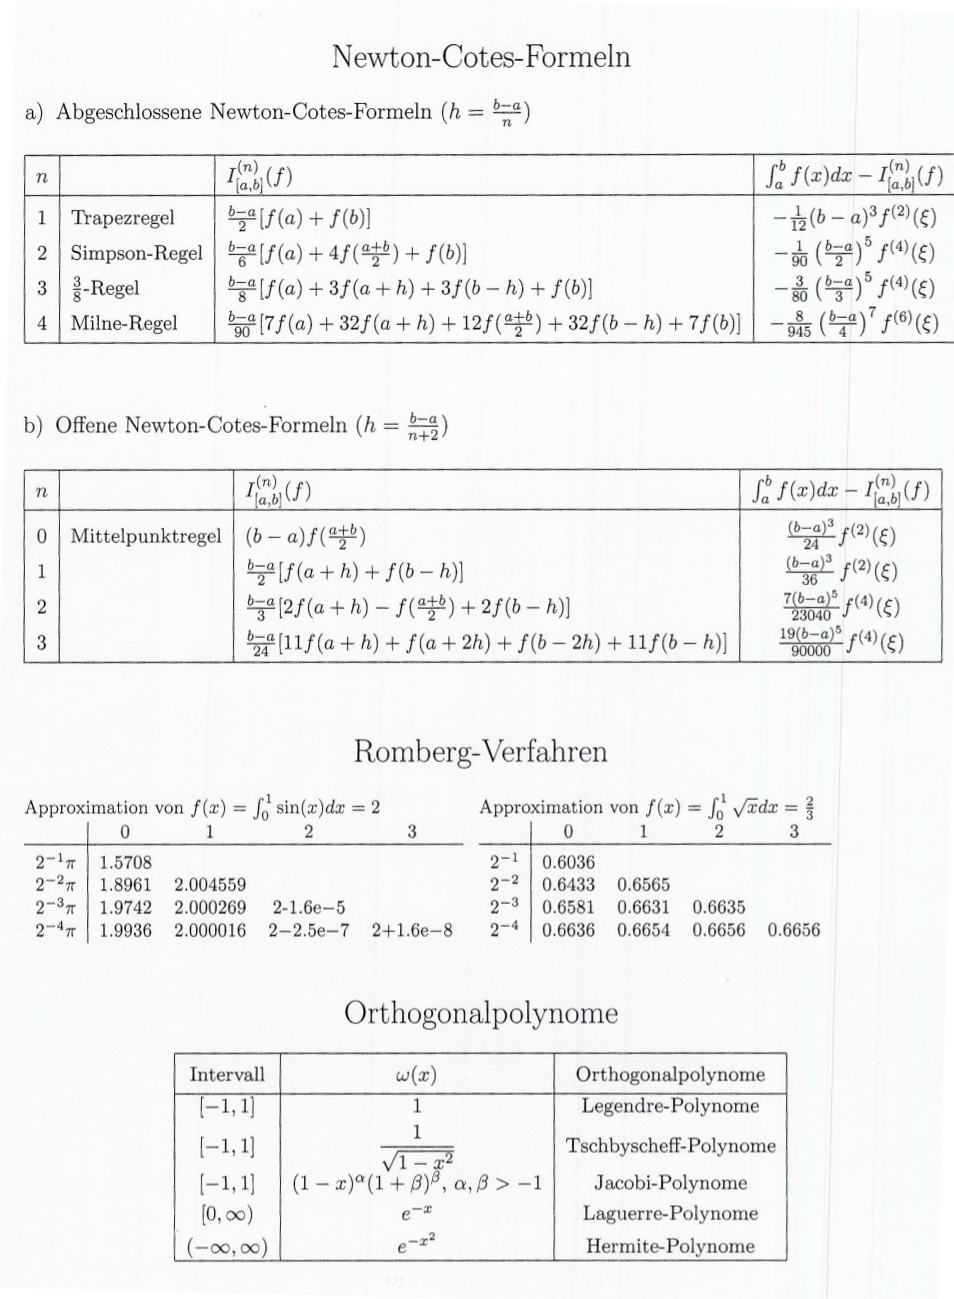
\includegraphics[width=\textwidth]{figures/num_int.png}
\end{figure}

\subsection{Gauß-Quadratur (Interpolatorische QF 2)}
Ziel: Formeln
\begin{align*}
  \int_a^b \omega(x) f(x) \dx \approx \sumizn{w_i f(x_i)}\;\;(a \leq x_0 < x_1 < \ldots < x_n \leq b)
\end{align*}
mit möglichst hohem Genauigkeitsgrad $m$, d.h. 
\begin{align*}
  \int_a^b \omega(x) p(x) \dx = \sumizn{w_i p(x_i)}\,\forall\, p \in \Pi_m
\end{align*}
wobei $\omega$ eine Gewichtsfunktion ist mit $\omega > 0$ in $(a,b)$ und $\omega$ nicht negativ in $[a,b]$.\\
QF über Interpolation von $f$ in $x_0 < \ldots < x_n$ durch $p_n \in \Pi_n$, d.h.
\begin{align*}
  \int_a^b \omega(x) p(x) \dx \approx \int_a^b \omega(x) p_n(x) \dx &= \int_a^b \omega(x) \sumizn{f(x_i)L_i(x) \dx} \\
  &= \sumizn{ f(x_i) \underbrace{\int_a^b \omega(x) L_i(x) \dx}_{w_i}}
\end{align*}
Obige Formel hat Genauigkeitsgrad von mindestens $n$. Genauigkeit ist maximal $2n+1$, denn für
\begin{align*}
  p(x) := \prod_{j=0}^n (x-x_j)^2 \in \Pi_{2n+2} \\
  \int_a^b \underbrace{\omega(x)}_{>0} \underbrace{p(x)}_{\geq 0,\not \equiv 0} \dx > 0\\
  QF = \sumizn w_i \underbrace{p(x_i)}_{=0} = 0
\end{align*}
$\Rightarrow$ QF für $p\,(\in \Pi_{2n+2})$ ist nicht exakt.\\
Konstruktion einer QF mit Genauigkeitsgrad $2n+1$ für $a \leq x_0 < x_1, \ldots < x_n \leq b$.
Sei $p \in P_{2n+10}$. Wähle $g \in \Pi_{2n+1}$ und führe Polynomdivision durch:
\begin{align*}
  p &= g \cdot q + r,\, q,r \in \Pi_n\\
  0 &\overset{!}{=} \int_a^b \omega(x) p(x) \dx - \sumizn{w_i p(x_i)} \\
  &= \underbrace{\int_a^b \omega(x) g(x) q(x) \dx}_{A} - \underbrace{\sumizn{w_i g(x_i) q(x_i)}}_{B} + \underbrace{ \int_a^b \omega(x) r(x) \dx - \sumizn{w_i r(x_i)}}_{=0}
\end{align*}
WÄHLE $g$ so, dass $A=0$ und $B=0$ ist.
\begin{align*}
  A \overset{!}{=} \int_a^b \omega(x) g(x) q(x) \dx = \inner{g}{q}_\omega
\end{align*}
$g \in \Pi_{n+1}\, q \in \Pi_n$. Wähle $g \perp \Pi_n \Rightarrow g \equiv \phi_{n+1}$ Orthogonalpolynom vom Grad $n+1$
\begin{align*}
  B \overset{!}{=} \sumizn{w_i \phi_{n+1}(x_i) q(x_i)}
\end{align*}
$\Rightarrow$ Wähle Nullstellen von $\phi_{n+1}$ als Stützstellen $x_0, \ldots,x_n$.
\para{Satz:} Wählt man als Stützstellen $x_0,\ldots,x_n$ die Nullstellen
des Orthogonalpolynoms $\phi_{n+1}$ bezüglich $\inner{.}{.}_\omega$ auf $[a,b]$, dann gilt:
\begin{enumerate}[a)]
  \item $\int_a^b f(x) \dx \approx \sumizn{w_i f(x_i)}$ mit
    \begin{align*} w_i = \int_a^b \omega(x) L_i(x) \dx \tag{Gauß-QF}\end{align*}
    hat Genauigkeit $2n + 1$
  \item Der Fehler der Formel ist \begin{align*}
      f^{(2n+2)}(\xi) \frac{1}{(2n+2)!} \int_a^b \omega(x) \prod_{i=0}^{n} (x-x_i)^2 \dx
    \end{align*} wobei $\xi \in [a,b]$ und $f \in C^{2n+2}[a,b]$ sein muss.
\end{enumerate}
Fehlerkonstante für $\omega(x) \equiv 1$\\
\begin{tabular}{ c | c | c | c}
  b-a & n=2 & n=4 & n=8 \\
  \hline
  4   &  2e-1 & & 3e-13\\
  2   &       & &      \\
  1   &       & &      \\
  0,5 & 7e-6  & 1e-12 & 1e-28\\
\end{tabular}\\
$\omega \equiv 1$ Gauß-Legendre-Quadratur\\
$\omega = \frac{1}{\sqrt{1-x^2}}$  Gauß-Tschebyscheff-Quadratur\\

Beispiel: Gauß-QF für $[a,b] = [-1,1],\, \omega \equiv 1$\\
$n=0$: $x_0$ ist Nullstelle von $P_1(x)=x$, Orthogonalpolynom $\in \Pi_1$ bzgl. $\inner{.}{.}_{\omega \equiv 1}$.\\
$x_0 = 0$ $w_0 = \int_{-1}^1 \underbrace{L_0(x)}_{\equiv 1} \dx = 2$\\
\begin{figure}[htbp]
  \centering
  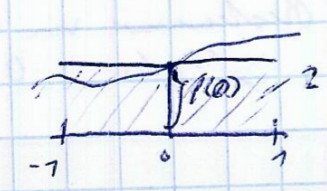
\includegraphics[width=0.2\textwidth]{figures/gauss_qf.png}
  \caption{Gauß-QF}
\end{figure}
$\int_{-1}^1 f(x) dx \approx 2 f(0)$ Mittelpunktformel\\

Transformation der Gauß-Legendre QF auf allgemeins Intervall $[a,b]$:\\
Seine $t_0,\ldots,t_n$ Stützstellen und $\tilde{w}_0,\ldots,\tilde{w}_n$ Gewicht für $[-1,1]$.\\
Transformation: 
\begin{align*}
  x:[-1,1] &\longrightarrow [a,b]\\
  t &\mapsto \frac{a+b}{2} + \frac{b-a}{2} t\\
  x(-1) = a && x(1) = b && \frac{\dx}{\dvar{t}} = \frac{b-a}{2} 
\end{align*}
\begin{align*}
  \int_{x(-1)=a}^{x(1)=b} f(x) \dx = \int_{-1}^1 f(x(t)) \frac{b-a}{2} \dvar{t} \approx
    \frac{b-a}{2} \sumizn{\tilde{w}_i f(x(t_i))}
\end{align*}
$\Rightarrow w_i = \frac{b-a}{2} \tilde{w}_i \qquad x_i = x(t_i)$

\subsection{Mehrdimensionale Integration (2D)}
Herkömmlicher Ansatz:
\begin{itemize}
  \item Zerlegung des Gebietes in einfache Elemente (Vierecke, Dreiecke) $B_i$
  \item Verwende Transformation $\psi_i: E \longrightarrow B_i$\begin{align*}
      \int_{B_i} g(x,y) \dx\dy = \int_E g(\psi_i(\tilde{x},\tilde{y})) \abs{\det J_i(\tilde{x},\tilde{y})} \dvar{\tilde{x}}\dvar{\tilde{y}}
  \end{align*} wobei $J_i$ die Jacobi-Matrix zu $\psi_i$ ist.
\end{itemize}
\subsubsection{Integration über das Einheitsquadrat}
\begin{align*}
  \int_0^1 \int_0^1 f(x,y) \dx\dy
\end{align*}
Sei $I_n(g) = \sumizn{w_i g(x_i)}$ QF im Eindimensionalen für $[0,1]$
\begin{align*}
  \int_0^1 \underbrace{\int_0^1 f(x,y) \dx}_{=:F(y)} \dy &= \int_0^1 F(y) \dy \approx \sumzn{j}{w_j F(x_j)} = \sumzn{j}{w_j \int_0^1 f(x, x_j) \dx}\\
    &\approx \sumzn{j}{w_j \sum_{i=0}^m w_i f(x_i, x_j) } := I_{n \times m}(f)
\end{align*}
Ist $I_m$ exakt vom Grad $M$, dann ist $I_{n \times m}$ exakt für alle Polynome\\
$p \in \mathrm{span} \{x^{k_1}y^{k_2}: 0 \leq k_1, k_2, \leq M\}$
\subsubsection{Interpolation über das Einheitsdreieck}
\begin{figure}[htbp]
  \centering
  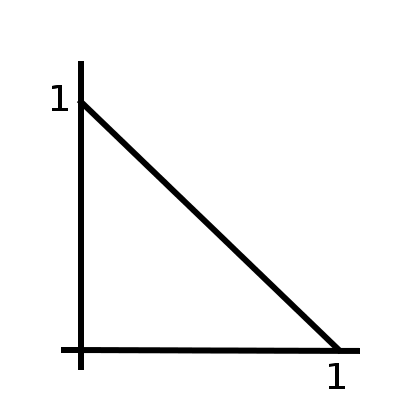
\includegraphics[width=0.3\textwidth]{figures/einheitsdreieck.png}
  \caption{Einheitsdreieck}
\end{figure}
Zwei Ansätze:
\begin{itemize}
  \item Duffy-Transformation: Idee: Transformation von QF für das Einheitsquadrat auf das Einheitsdreieck.
  \item Bestimmung von QF über den Ansatz: Alle Monome der Form $x^{k_1}y^{k_2} \qquad 0 \leq k_1, k_2, \leq M$
    sollen exakt integriert werden.
\end{itemize}
